\documentclass[conference]{IEEEtran}
%future work: local patch operator
%complexity

\usepackage{subfig}
\usepackage{wrapfig}
\usepackage{amsmath}
\usepackage{url}
\usepackage{pifont}
%\usepackage{times}
\usepackage{rotating}
%\usepackage{balance} 
\usepackage{color, colortbl}
\usepackage{graphicx}
\usepackage{algorithmicx}
\usepackage[running]{lineno}
\usepackage{program}
\usepackage{cite}
\usepackage{alltt}
\usepackage{balance}
\newcommand{\eq}[1]{Equation~\ref{eq:#1}}
\newcommand{\bi}{\begin{itemize}}
	\newcommand{\ei}{\end{itemize}}
\newcommand{\be}{\begin{enumerate}}
	\newcommand{\ee}{\end{enumerate}}
\newcommand{\tion}[1]{\textsection\ref{sec:#1}}
\newcommand{\fig}[1]{Figure~\ref{fig:#1}}
\definecolor{lightgray}{gray}{0.975}
\usepackage{fancyvrb}
\usepackage{stfloats}
\usepackage{multirow}
\usepackage{listings}
\usepackage{amsmath}  
\DeclareMathOperator*{\argmin}{arg\,min} 
\DeclareMathOperator*{\argmax}{arg\,max} 
%\usepackage[usenames]{xcolor}




\usepackage{color}
\newcommand{\colorrule}[1]{\begingroup\color{#1}\hrule\endgroup}

\definecolor{darkgreen}{rgb}{0,0.3,0}

\usepackage[table]{xcolor}
\definecolor{Gray}{rgb}{0.88,1,1}
\definecolor{Gray}{gray}{0.85}
\definecolor{Blue}{RGB}{0,29,193}
\newcommand{\G}{\cellcolor{green}}
\newcommand{\Y}{\cellcolor{yellow}}


\definecolor{MyDarkBlue}{rgb}{0,0.08,0.45} 
\newenvironment{changed}{\par\color{MyDarkBlue}}{\par}

\newcommand{\ADD}[1]{\textcolor{MyDarkBlue}{{\bf #1}}}
\newcommand{\addit}[1]{\begin{changed}\input{#1}\end{changed}}

\usepackage{color}
\usepackage{listings}
\usepackage{setspace}

\definecolor{Gray}{gray}{0.9}
\newcommand{\kw}[1]{\textit{#1}}
\newcommand{\quart}[4]{\begin{picture}(75,6)
	{\color{black}\put(#3,3){\circle*{2.5}}\put(#1,3){\line(1,0){#2}}}\end{picture}}
% New Commands

\definecolor{Code}{rgb}{0,0,0}
\definecolor{Decorators}{rgb}{0.5,0.5,0.5}
\definecolor{Numbers}{rgb}{0.5,0,0}
\definecolor{MatchingBrackets}{rgb}{0.25,0.5,0.5}
\definecolor{Keywords}{rgb}{0,0,1}
\definecolor{self}{rgb}{0,0,0}
\definecolor{Strings}{rgb}{0,0.63,0}
\definecolor{Comments}{rgb}{0,0.63,1}
\definecolor{Comments}{rgb}{0.5,0.5,0.5}
\definecolor{Backquotes}{rgb}{0,0,0}
\definecolor{Classname}{rgb}{0,0,0}
\definecolor{FunctionName}{rgb}{0,0,0}
\definecolor{Operators}{rgb}{0,0,0}
\definecolor{Background}{rgb}{1,1,1}
\title{Actionable = Cluster + Constrast?}

% You can go ahead and credit any number of authors here,
% e.g. one 'row of three' or two rows (consisting of one row of three
% and a second row of one, two or three).
%
% The command \alignauthor (no curly braces needed) should
% precede each author name, affiliation/snail-mail address and
% e-mail address. Additionally, tag each Slope of
% affiliation/address with \affaddr, and tag the
% e-mail address with \email.
%
% 1st. author
\author{Rahul Krishna, Tim Menzies\\
	Computer Science, North Carolina State University, USA\\
	\{i.m.ralk, tim.menzies\}\@gmail.com
	
	% use '\and' if you need 'another row' of author names
	% 4th. author
}


\pagestyle{plain}
\begin{document}
<<<<<<< HEAD
	\maketitle
	\begin{abstract}
		There are many
		algorithms for data {\em classification} such as  C4.5, Naive Bayes, SVM, etc.
		Are these enough for software data analytics? Or should we be supporting
		another kind of reasoning? For example, this paper does not answer 
		``what is'' (i.e. the standard classification problem), but instead  offers advice on ``what to change''.
		Two approaches for learning minimal, yet effective,  changes,  software
		artifacts are explored. Lessons learned are reported.
	\end{abstract}
	\begin{IEEEkeywords}
		Prediction, case-based reasoning, data mining, software engineering.
	\end{IEEEkeywords}
	
	\section{Introduction} 
	How should we handle ``unpopulular'' results
	for data analytics? For example, if a business manager is presented
	with a data mining result that troubles them (e.g. an estimate of
	development time that is distressingly long), what advice
	can we offer them on management actions to {\em change} hat estimate?
	
	This is an important question, and one with much currency in industry.
	In the summer of 2011 and 2012, one of us (Menzies) spent two months
	working on-site at Microsoft Redmond,
	observing data mining analysts.  He
	noted how Microsoft's data scientists
	discussed their data with  business users. 
	One surprising from that study was just how
	little time was spent  
	inspecting  of the output of data miners as compared to another process, which we call {\em peeking}.
	In {\em peeking}, analysts and users spend much time
	inspecting and discuss small samples of either raw or exemplary or synthesized project data.  Further, very little of those discussions were  focused on classification
	(the additional of a labels to some unlabelled data). Rather, much time
	was spent in those meetings discussion {\em what to do next}; i.e. trying
	to determine what could be altered to better improve some business outcome.
	
	That   Microsoft  stufy found two common ``peeking'' methods.
	In {\em data engagement meetings},
	users debated the implications of data
	displayed on a screen. In this way, users
	engaged with the data and with each other by
	monitoring each others' queries and check each others'
	conclusions.
	
	Another data analysis pattern observed
	at Microsoft was  {\em cluster + contrast} in which
	data is  reduced to a few
	clusters. Users are then just shown the delta between those
	clusters. While contrasting, if feature values are
	the same in both clusters, then these were pruned from
	the reports to the user. In this way, very large
	data sets can be shown on one PowerPoint
	slide. Note that {\em cluster+contrast} was a tool that can be usefully employed within
	{\em data engagement meetings}.
	
	
	Cluster+contrast and engagement
	meetings are common practices at Microsoft. Yet  these methods had never been rigorously studied or certified.
	For both those reasons,
	we reflected over those tools to discover and analyze their
	underlying process. The result was HOW: a tool
	that combines two
	data reduction methods:\bi
	\item Method1: feature selection
	\item Method2: centroid generation from   clusters.
	\ei
	While Method1 is widely used~\cite{Menzies2010},
	to the best of our knowledge, this combination has not been thoroughly explored before.
	Hence, this paper explores ``peeking''.
	
	\section{How to Cluster}
	Recent results suggest  we are free to select from a wide range of 
	clustering methods.  Ganesan~\cite{div14} explored 
	different clustering methods for SE data using   effort and defect data from
	the PROMISE repository\footnote{http://openscience.us/repo};
	That studied explored
	K-Means, mini-batch-K-Means, DBscan, EM, Ward, and the WHERE algorithm discussed
	below.
	Clusters were assessed via the performance of prediction 
	learned from the clusters by Random Forests (for defect prediction)
	and M5prime or linear regression (for effect estimation).  Ganesan found
	that the details of the clustering method were less important than ensuring that  a large number of clusters were generated.
	
	Accordingly, we select a clustering method that generates $\sqrt{N}$ clusters
	from $N$ examples, that runs fasts, which has shown promise in prior work~\cite{Menzies2013}, and which ignores spurious dimensions (the last item is important since, in our experience, much SE data is ``noisey''; i.e. contains signals not associated with the target variable). For the rest of this article,
	we use  the top-down
	bi-clustering method described in \fig{where} which recursively divides the
	data in two  using a dimension that captures the greatest variability in the data. 
	\begin{figure}[t]
		\small
		~\hrule~
		
		{\bf Top down clustering using WHERE:}
		
		The data is recursively divided in clusters using WHERE as follows:
		\begin{itemize}
			
			\item Find   two   distance cases,  $X,Y$
			by picking any case $W$ at random, then setting $X$ to its most
			distant case, then setting $Y$ to the case most distant from
			$X$~\cite{fastmap}
			(this requires only $O(2N)$ comparisons
			of $N$ cases).
			\item Project each case $Z$
			onto a {\tt Slope} that  runs between $X,Y$ using the cosine
			rule. 
			\item Split the data at the median $x$ value of all cases and
			recurses on each half  (stopping when
			one half has less  than $\sqrt{N}$ of the original population).
		\end{itemize}
		~\hrule~
		
		{\bf Constructing Decision Trees:}
		
		A decision tree is built using CART with entropy being used to generate splits in the data. The leaf nodes of the tree are weighted by measuring the mean of majority cluster of the leaf. To limit the size of the tree Features are pruned using information gain.
		
		~\hrule~
		
		{\bf Generating contrast sets:}
		\begin{itemize}
		\item Identify current position on the tree.
		\item Identify the nearest ``Better'' branch.
		\item Identify the ``Delta'' between the cluster.		
		\end{itemize}
		~\hrule~
		\caption{A summary of Contrast Trees}
		\label{fig:contast_trees}
	\end{figure}
	
	\section{How to Contrast}
	Once we have  clusters, the next task is to offer business users lessons learned from comparing different clusters.
	
	Once methods for doing so is a {\em contrast tree}.
	First, we cluster the data to find clusters $C_1,C_2,...$.
	Next, using those clusters as class labels, we execute a decision tree algorithm to find what attributes select for different clusters. Next, to learn recommendations for a business user, we ask (1) what {\em current} cluster are you in?; (2) what {\em desired} cluster do you want to move to?; (3) what is the delta between those clusters? To answer the last question, we report the delta in the branches of the decision tree that lead to {\em current} and {\em desired}. 
	
	%Contrast trees are decision trees that can be used to learn decision rules from a large data set. The use of decision trees for this purpose makes it easy to visualize the data and also makes interpretation of the recommended policies fairly straight forward. In addition to this, contrast tree generate ranges of decisions that allow for better feasibility.
	\subsection{How does a contrast tree work?}
	Contrast trees works by building a simple decision tree based on entropy, as in the classification and regression trees. Contrast tree uses the WHERE clustering algorithm, which in-turn uses FASTMAP \cite{} to compute clusters 
	that contain instances that are spatially close. Each cluster is assigned a unique cluster id. Then, a simple decision tree is built using a standard classification and regression tree (CART). The tree is built with the following tunable features:
	\begin{itemize}
		\item \textit{Entropy} is used as criteria for generating optimum cuts while building the decision trees. These were shown to be consistent in giving high performance across most data.
		\item \textit{Minimum samples per leaf} defines the minimum number of instances in a leaf of the decision tree.
		\item \textit{Max depth} defines the number of levels of recursive splits that are allowed in the tree.
	\end{itemize}
	Decision trees can be used to generate a decision rule, which when applied to solution sets must theoretically improve performance. To generate rules -- a tree is constructed with some training data, and for every instance in a the test data, we find a branch in the tree that best matches the test data. All instances that needs improvement in the test data constitute the ``worst'' set W. We find the nearest branch, ``B'', in the tree with better performance. The difference between W and B constitutes the decision rules.
	
	A contrast set, ``C'' is simply a collection of all the decision rules. It can be obtained traversing through the tree from ``W'' to ``B'' and tracking all the branch variables along this path. Note that the branch variables use decision ranges instead of single point solutions, making implementation of the rules in real life feasible. 
	
	\subsection{Why would it work?}
	Contrast set seemed like it would be a fine tool for generating decision rules. They present some key advantages which are listed below:l
	\begin{itemize}
		\item They allow the user to exert a fine grain control over the parameters that needs to be changed, while providing a way to visualize the recommended changes.
		\item The changes suggested by the contrast sets are inherently local in nature, making the changes practical and potentially easy to implement.
		\item The contrast tress require a worst case time complexity of $O(n)$, which is a function in linear time.
	\end{itemize}

	\begin{figure}[t]
		{\footnotesize  \begin{tabular}{{llrrc}}
				\arrayrulecolor[gray]{.90}
				\rowcolor[gray]{.95} \textbf{Rank} & \textbf{Treatment} & \textbf{Median} & \textbf{IQR} & \\
				1 &     Ant (Tree) &    0.67  &  0.41 & \quart{0}{39}{37}{69} \\
				1 &   Jedit (Tree) &    0.68  &  0.13 & \quart{36}{13}{38}{69} \\
				1 &     Ant (WHAT) &    0.7  &  0.13 & \quart{33}{13}{40}{69} \\
				1 &   Jedit(WHAT) &    0.72  &  0.25 & \quart{25}{24}{42}{69} \\
				\hline \end{tabular}}
	\caption{Results comparing the performance scores on sample projects from the Jurezcko data sets.}
	\end{figure}
	
	
	\begin{figure*}[!t] 
		\begin{minipage}{0.5\linewidth}
			\subfloat[Tree Learner]{
				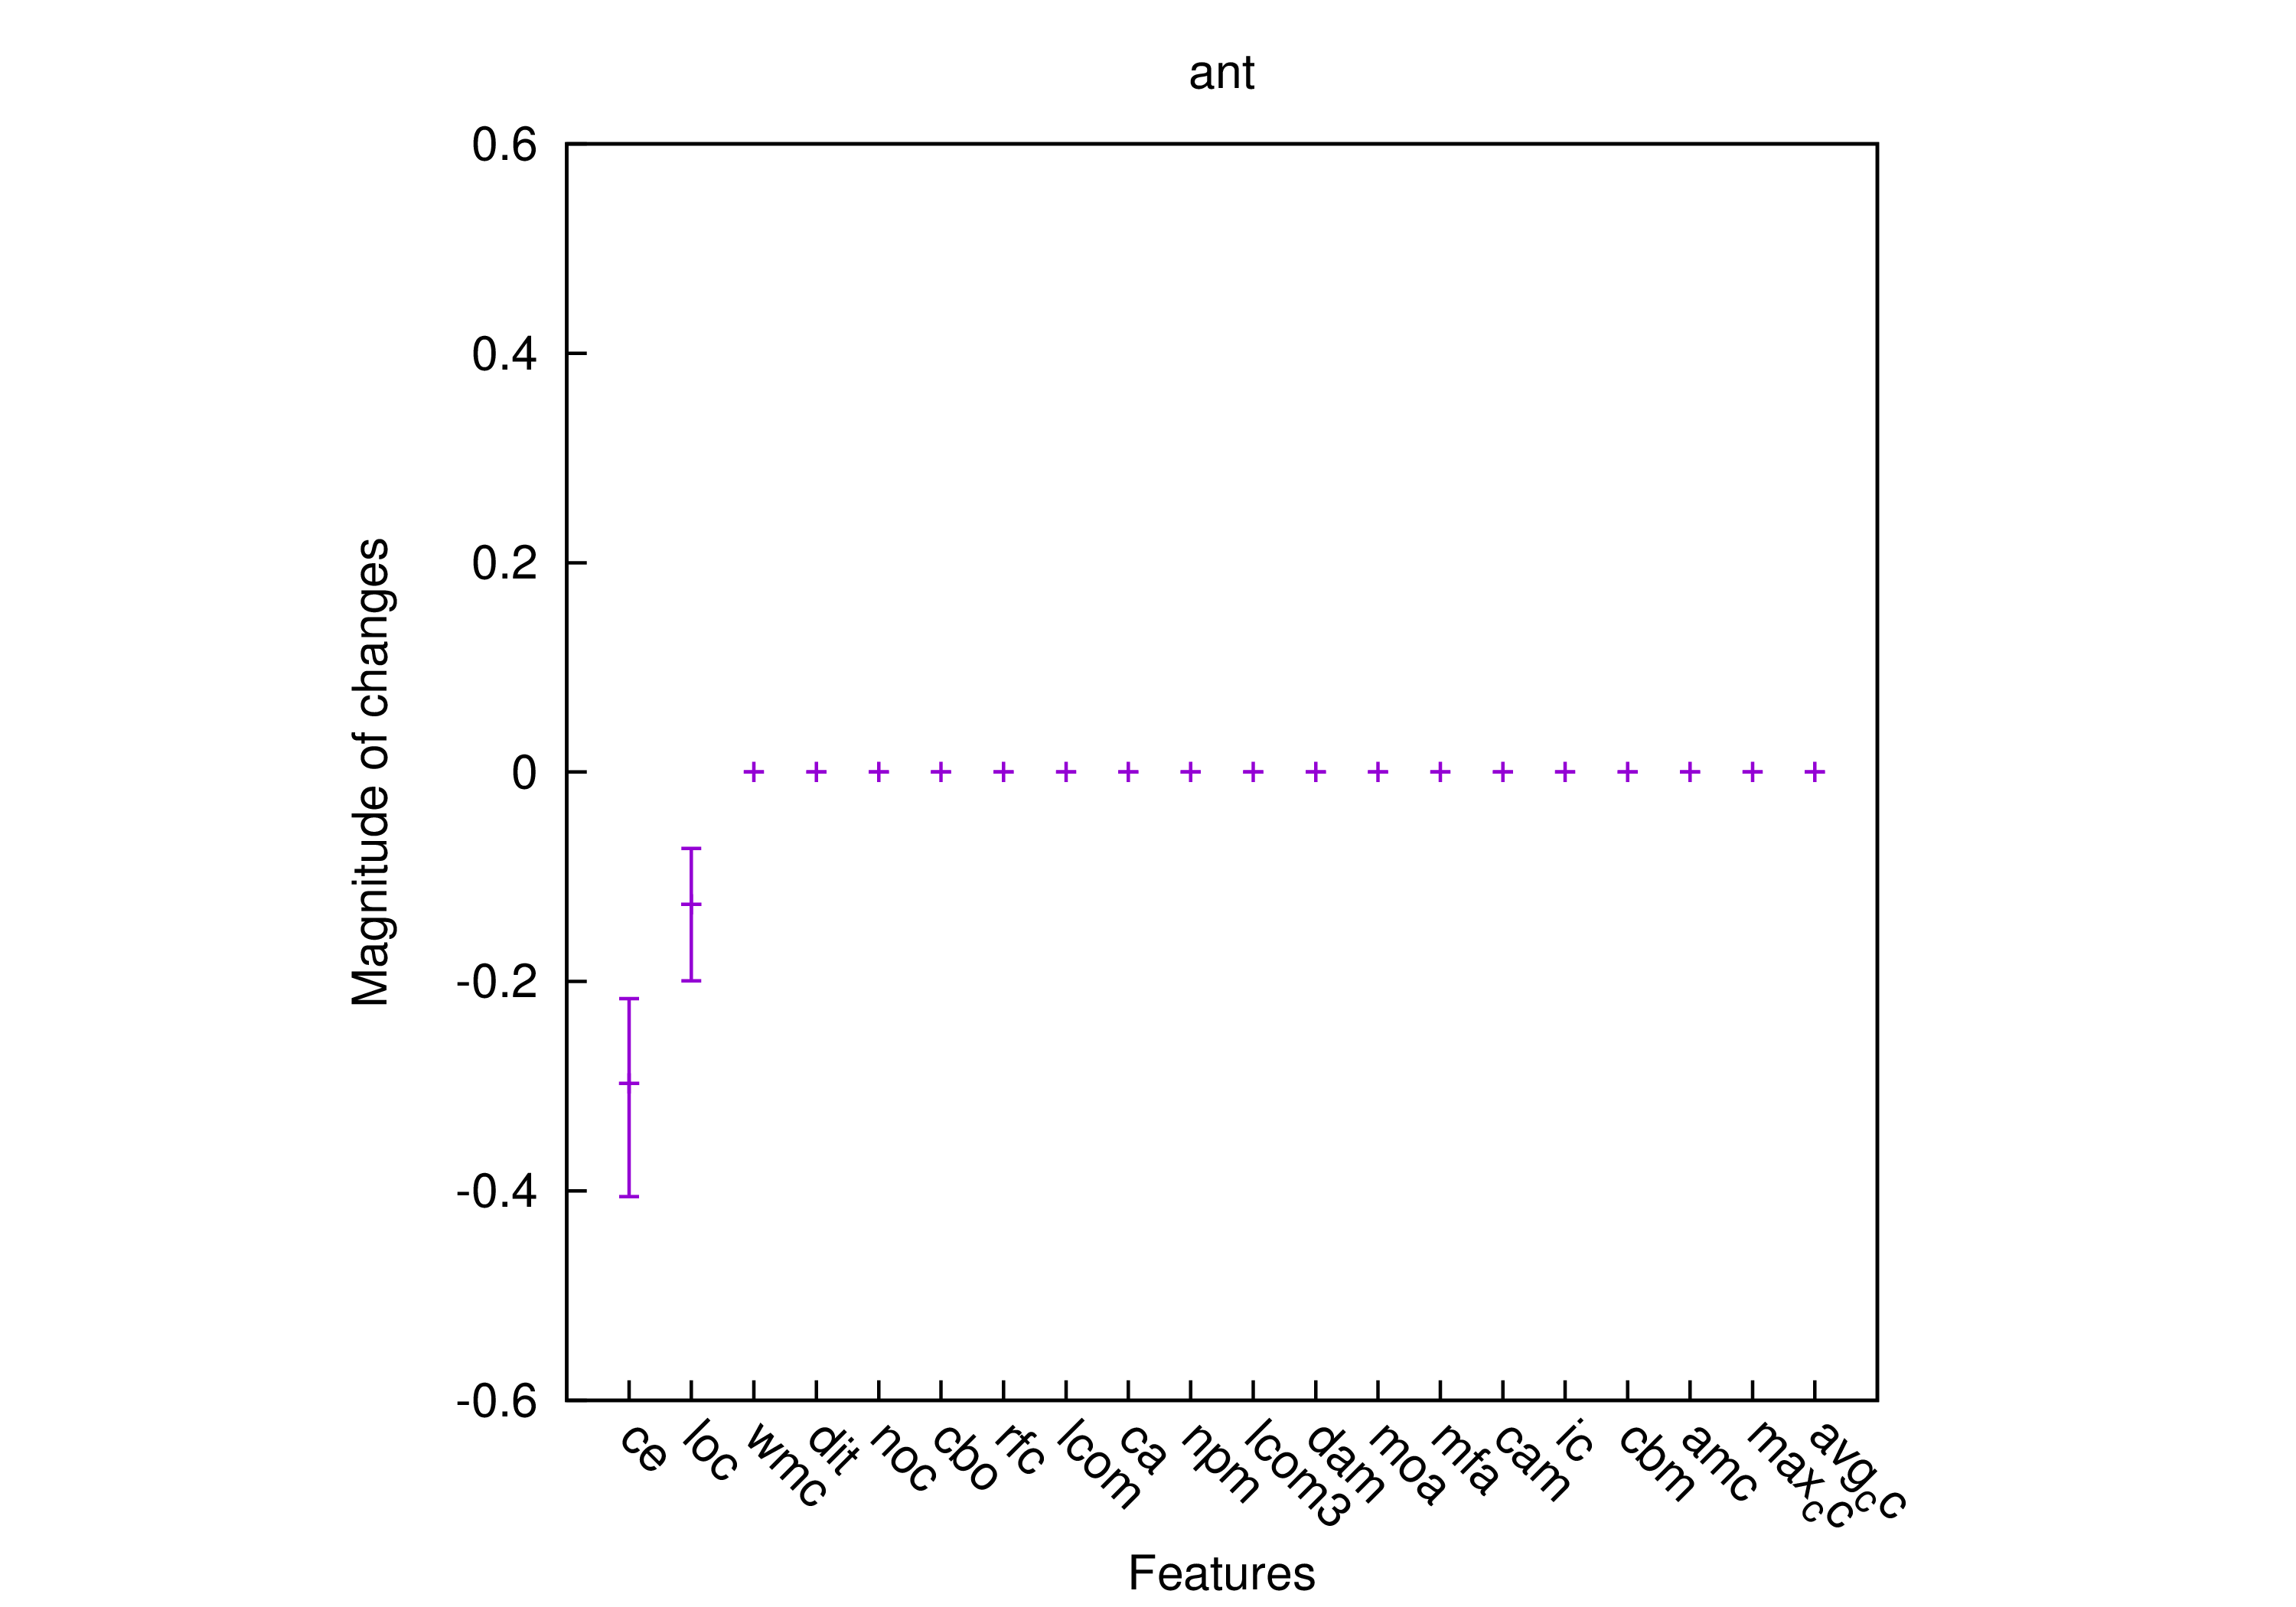
\includegraphics[width=\linewidth]{ant1.png}
				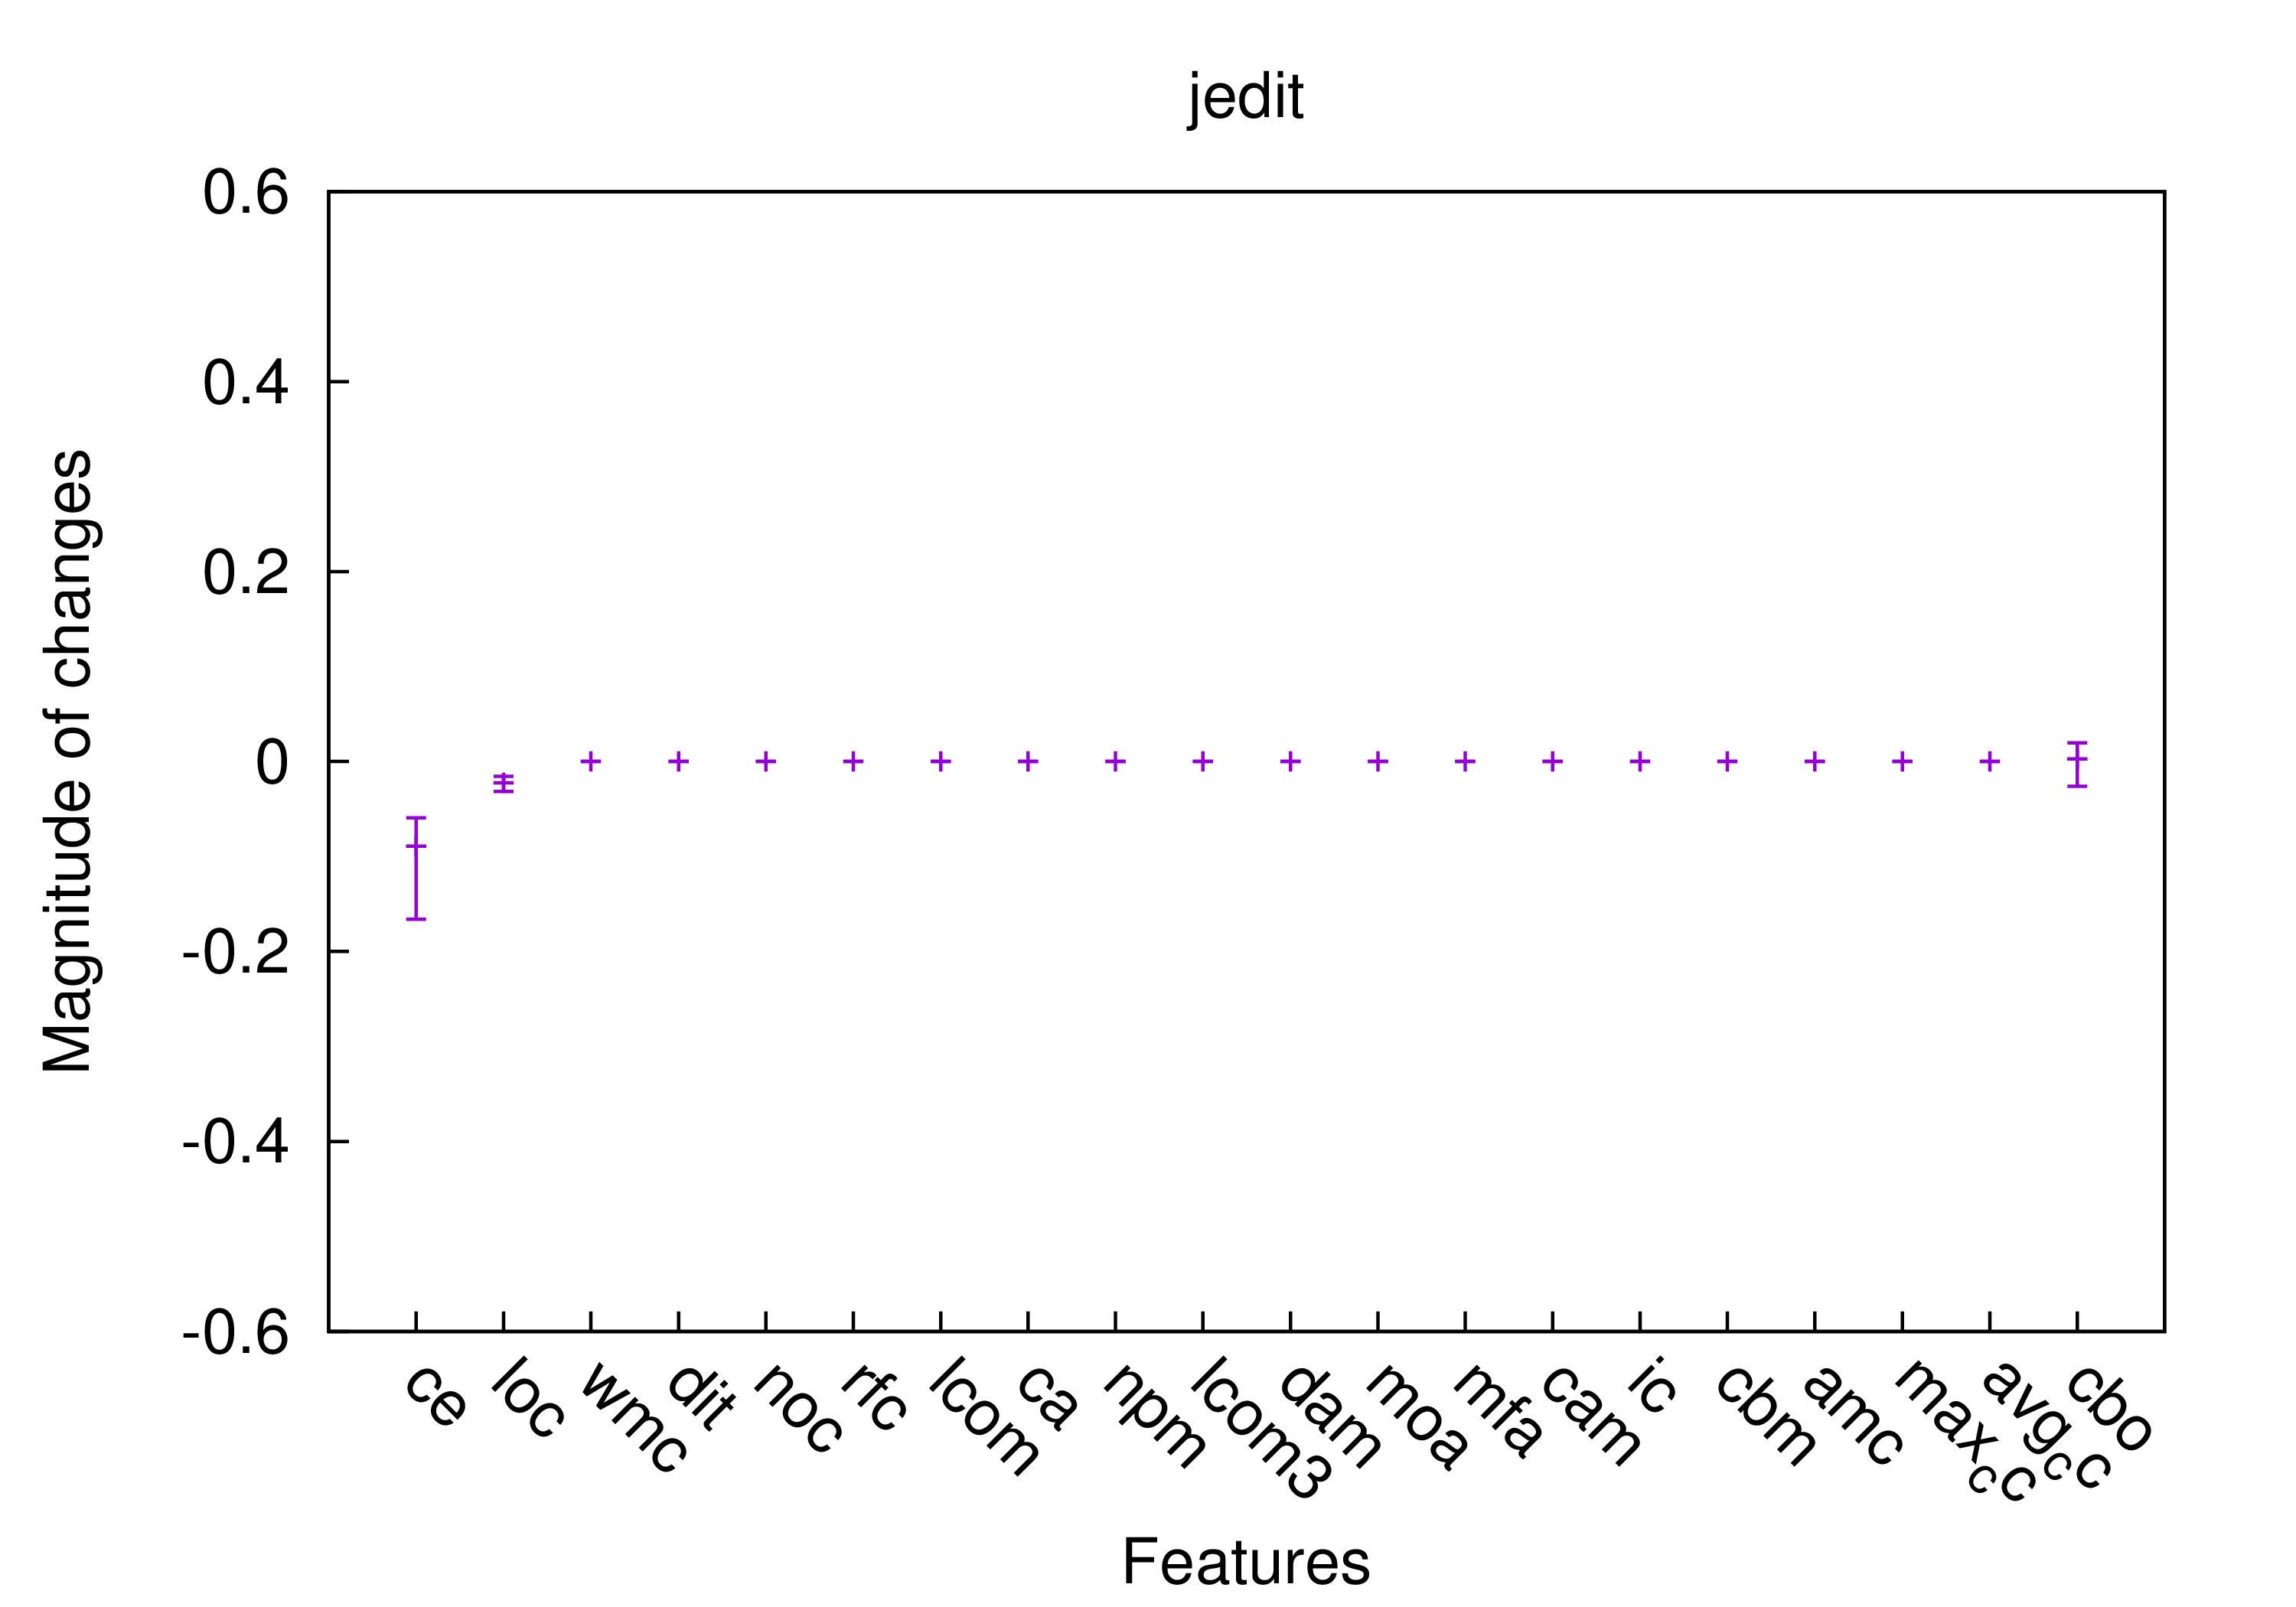
\includegraphics[width=\linewidth]{jedit1.png}}\\
			\subfloat[WHAT]{			
				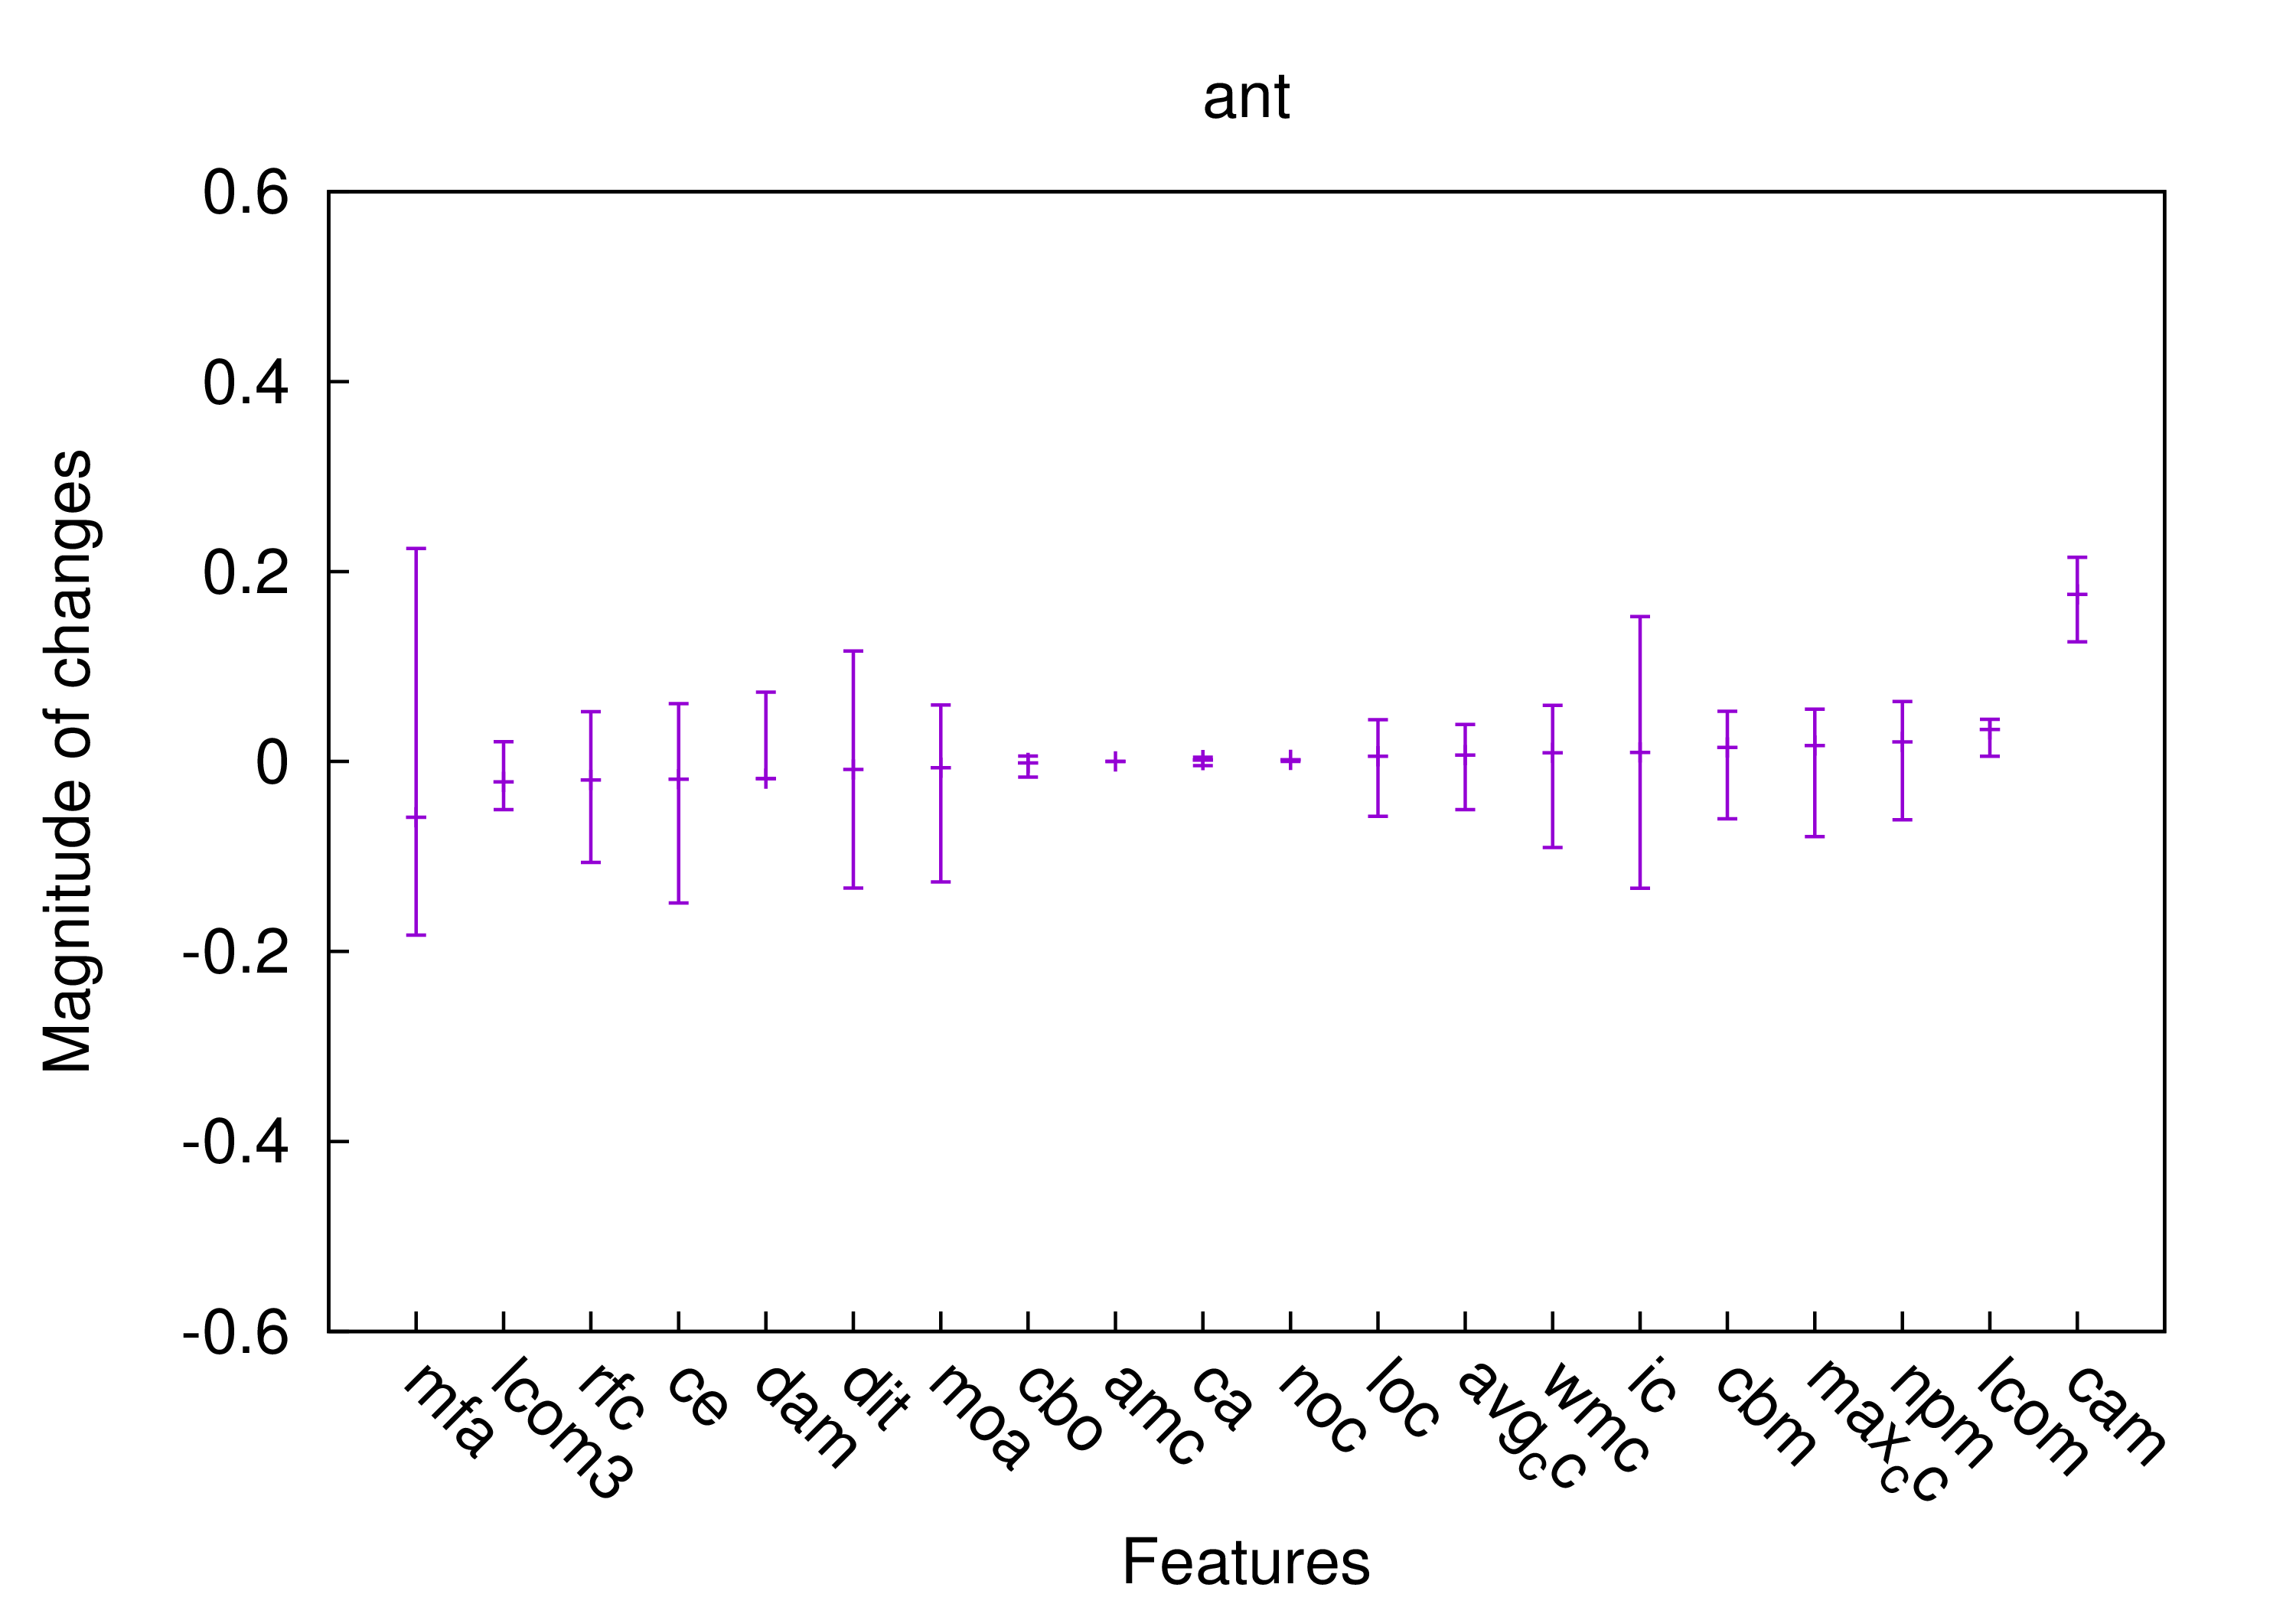
\includegraphics[width=\linewidth]{ant2.png}
				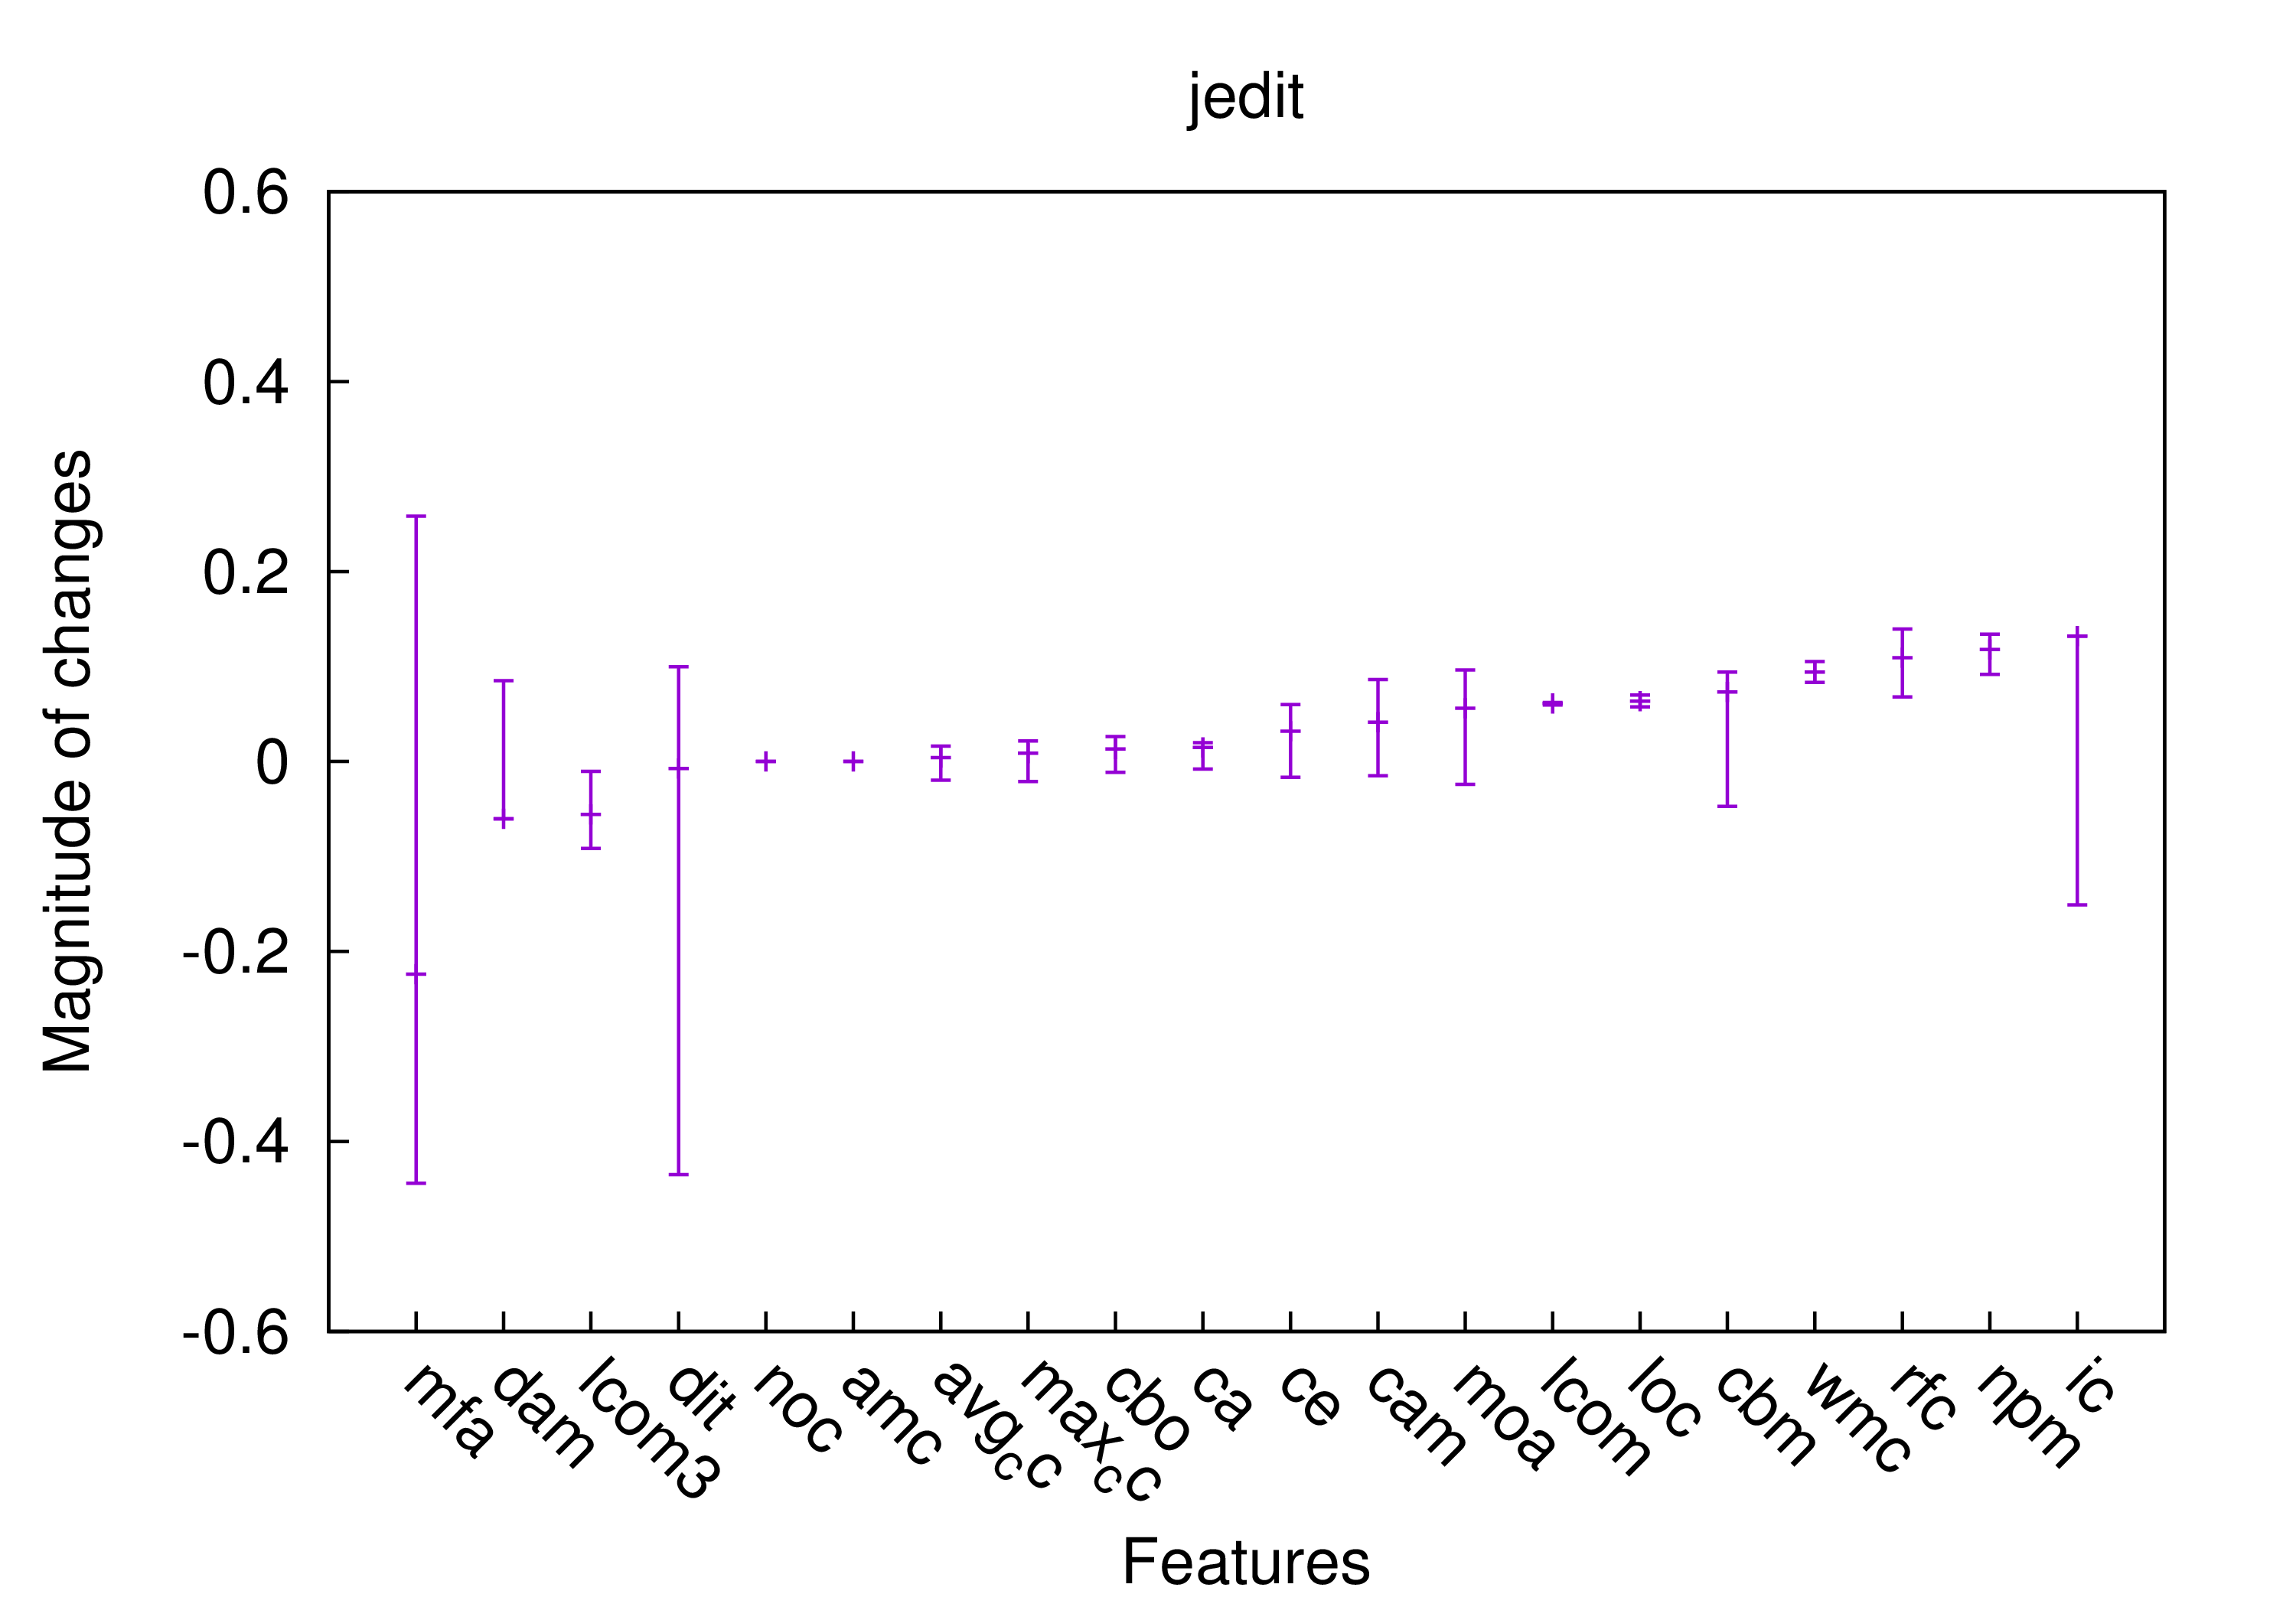
\includegraphics[width=\linewidth]{jedit2.png}}
		\end{minipage}
		\caption{Performance Comparision}
	\end{figure*}
	
	\subsection{Reasons for failure}
	Although the idea seemed ideal, initial implementation of the contrast tree provided results that were discouraging. One of the major problems with using contrast trees was that the trees were rather large. The initial motivation was that the trees could serve as a medium for experts to identify and explore solution spaced that were local to the problem. The size of the decision tree jeopardized the readability of the solutions by increasing the complexity. In our efforts to reduce the size of the tree, we devised a pruning method, that prunes away irrelevant branches that do not contribute better solutions. The smaller trees, while being easier to understand, posed another problem: the test instances were too dissimilar to the leaves in the tree. This meant that the relevance of the contrast set could not be justified.
	
	The depth of the tree also influences the performance of contrast sets. The depth is represented by levels of splits in the tree, and this parameter determines the number of features that require changes. If the tree is too shallow, the changes suggested by the planner are too little to make any difference. On the other hand, deeper trees leads to over-fitting and therefore suggests too many changes when not required.
	
	A study was conducted on numerous examples of the Jureczko object-oriented static code data sets \cite{}: Ant, Camel, Ivy, Jedit, Log4j, Lucene, Poi, Synapse, Velocity, Xalan, Xerces \footnote{Available from the object-oriented defects section of the PROMISE respository openscience.us/repo/defect/ck.}. On these data sets, the plans generated by contrast tree advise
	how to change static code attributes in order to reduce defects in Java classes. The challenges with contrast trees had a profound impact on the performance, as shown in figure \ref{}.
	\subsection{What worked?}
	Contrast tree is the second generation of our efforts to use contrast set learners for planning case based reasoning. W2 represents the first generation of our work. W2 is a CBR planner that reflected over the delta of raw attributes \cite{}. However, it frequently suffered from an optimization failure. When its plans were applied, performance improved in only  $\tfrac{1}{3}$rd of test cases. 
	
	Generation two of our work resulted in the development of contrast trees. It uses a recursive clustering method discussed above followed by summarizing these recursive divisions into a tree structure. Although the initial results with contrast tree were weak, they were somewhat positive. We tried to extend and improve the contrast tree prototype, however the results were not encouraging. The tree-based approach suffered from one key issue: the local changes were highly ineffective in reducing the defects, see figure \ref{}. In addition, it also faced the optimization failure problem, which was also seen with W2. 
	
	As a continuation of the contrast tree work, we built HOW as a simpler approach that was to provide a baseline result, above which contrast tree was meant to do better. However, HOW’s results were so good that we threw away months of work on tree-based planning with contrast tree. 
	\section{Future Work}
	Now, we strongly recommend HOW over contrast tree (and W2) since, as shown by the following results, HOW’s plans never lead to performance getting worse. Also, when HOW did improve the expected values of the performance, those performance improvements were an order of magnitude larger than those seen with contrast tree. 
\bibliographystyle{plain}
\bibliography{hownot}
\end{document}